\documentclass[dvipdfmx, twocolumn, a4paper]{hcresume}

\usepackage{epsfig}
\usepackage{amsmath}
\usepackage{graphics}
\usepackage{graphicx}
\usepackage{txfonts}
\usepackage{color}
\usepackage{BoldGothic4fig}
\usepackage{bm}
\usepackage{verbatim}
\usepackage{wrapfig}
\usepackage{ascmac}
\usepackage{makeidx}
\usepackage{enumerate}
\usepackage{comment}
\usepackage{multirow}
\usepackage{listings}

\usepackage[hang,small,bf]{caption}
\usepackage[subrefformat=parens]{subcaption}

%
\def\linesparpage#1{\baselineskip=\textheight
   \divide\baselineskip by #1}
\def\kcharparline#1{%
   \ifx\xkanjiskip\undefined%
   \jintercharskip 0mm plus 0.2mm minus 0.2mm
   \else
   \xkanjiskip 0mm plus 0.2mm minus 0.2mm
   \fi
   \settowidth{\textwidth}{}%
   \multiply\textwidth by #1}
%
\newcommand\figref[1]{\textbf{図~\ref{fig:#1}}}
\newcommand\tabref[1]{\textbf{表~\ref{tab:#1}}}
\newcommand{\bhline}[1]{\noalign{\hrule height #1}}

\hcheader{MIプログラム 卒研中間発表会}
\title{\bf 評価者特性の時間変動を考慮した項目反応モデル}
\author{1810519 林真由}
\supervisor{指導教員 宇都 雅輝 准教授}

\begin{document}
\maketitle
\pagestyle{empty}
\thispagestyle{empty}
\section{はじめに}
近年,大学入試や資格試験,教育評価などの場において,パフォーマンス評価は重要な役割を果たしている.その中で,パフォーマンス評価では,評価者の厳しさや一貫性の違い,各得点の使用傾向の差などにより,採点に偏りが生じ,受検者の能力を正確に測ることができないという問題が発生することがある.この問題を解決するために項目反応理論(Item response theory:IRT)\cite{IRTLord}と呼ばれる数理モデルの利用が近年注目されている.

多くのモデルでは,課題と評価者の特性を考慮した能力推定を行うことができるが,これらのモデルは評価者の特性が評価中に変化しないという仮定のもと成り立っている.しかし,その仮定は現実には成り立たないことがある.この評価者の採点基準が採点過程で変化する特性は評価者ドリフト(Rater Drift)と呼ばれ,これを考慮したモデルについても提案がなされている.既存モデルでは,一定の時間区分ごとの評価者の厳しさパラメータを導入することで,評価者特性の時間変化を捉えるモデルとなっているが,このモデルでは各時間区分ごとのパラメータが独立しているため,パラメータの推定が難しいと言う問題点がある.

この問題を解決するために,本研究では,時間区分ごとの評価者の厳しさにマルコフ性を仮定した新しい項目反応モデルを提案する.また,シミュレーション実験と実データ実験を通して提案モデルの有効性を示す.

\section{項目反応理論}
本研究は,課題・評価者・時間の特性を考慮した高精度な能力推定を行うことを目的とする.このような能力推定を実現するために,本研究ではIRTを利用する.

現在最も評価者特性を柔軟に表現できる項目反応モデルとして,一般化多相ラッシュモデルが知られている\cite{g-MFRM}.
このモデルでは,評価者$r$が課題$i$における受検者$j$のパフォーマンスに評点$k$を与える確率を次式で定義する.
\begin{displaymath}
  P_{ijrk}=\frac{\mathrm{exp}\sum_{m=1}^{k}\{\alpha_i\alpha_r(\theta_{j}-(\beta_{i}+\beta_{r})-d_{rm})\}}{\sum_{l=1}^{K}\mathrm{exp}\sum_{m=1}^{l}\{\alpha_i\alpha_r(\theta_{j}-(\beta_{i}+\beta_{r})-d_{rm})\}}
\end{displaymath}
ここで,$d_{rm}$は評価者$r$のスコア$k$に対する厳しさを表すステップパラメータである.モデルの識別性のために,$\sum^{I}_{i=1}{\mathrm{log}\alpha_i}=0,\sum^{I}_{i=1}{\beta_i}=0,\sum^{K}_{k=2}{d_{rk}}=0, d_{r1}=0$を仮定する.

上記のモデルでは,課題と評価者の特性を考慮した能力推定を行うことができるが,これらのモデルは評価者の特性が評価中に変化しないという仮定のもと成り立っている.しかし,実際には評価の仮定で特性が変化する評価者ドリフトが生じる場合がある.
評価者特性の時間変化を考慮できるモデルとして,RaudenbushとBryk\cite{Raudenbush}は,評価者の厳しさの安定性を調べるために,時間$t$における評価者$r$の厳しさの変化を反映させるモデルを次の式で提案した.
\begin{displaymath}
  P_{ijrtk}=\frac{\mathrm{exp}\sum_{m=1}^{k}(\theta_{j}-\beta_{r} - \pi_{r}\beta_{rt}-d_{m})}{\sum_{l=1}^{K}\mathrm{exp}\sum_{m=1}^{l}(\theta_{j}-\beta_{r} - \pi_{r}\beta_{rt}-d_{m})}
\end{displaymath}
ここで,$\beta_{r}$は評価者$r$の初期の厳しさ,$\pi_{r}$は評価者$r$の厳しさの変化の傾き,$\beta_{rt}$は評価者$r$の時刻$t$における時間区分を表す.

評価者ドリフトを考慮した項目反応モデルでは,一連の採点データを一定の時間区分で区切り,時間区分ごとの評価者パラメータを導入する.具体的には,図\ref{timeid}のように,評価者が学習者を評価する順番が早い順にデータを並べ,早い方から時間区分数に分割し,時間区分を表すインデックス(以降ではTimeIDと呼ぶ)を付与する.時間区分ごとのデータ数は,学習者数を時間区分数で割った数になる.
\begin{figure}[t]
  \centering
  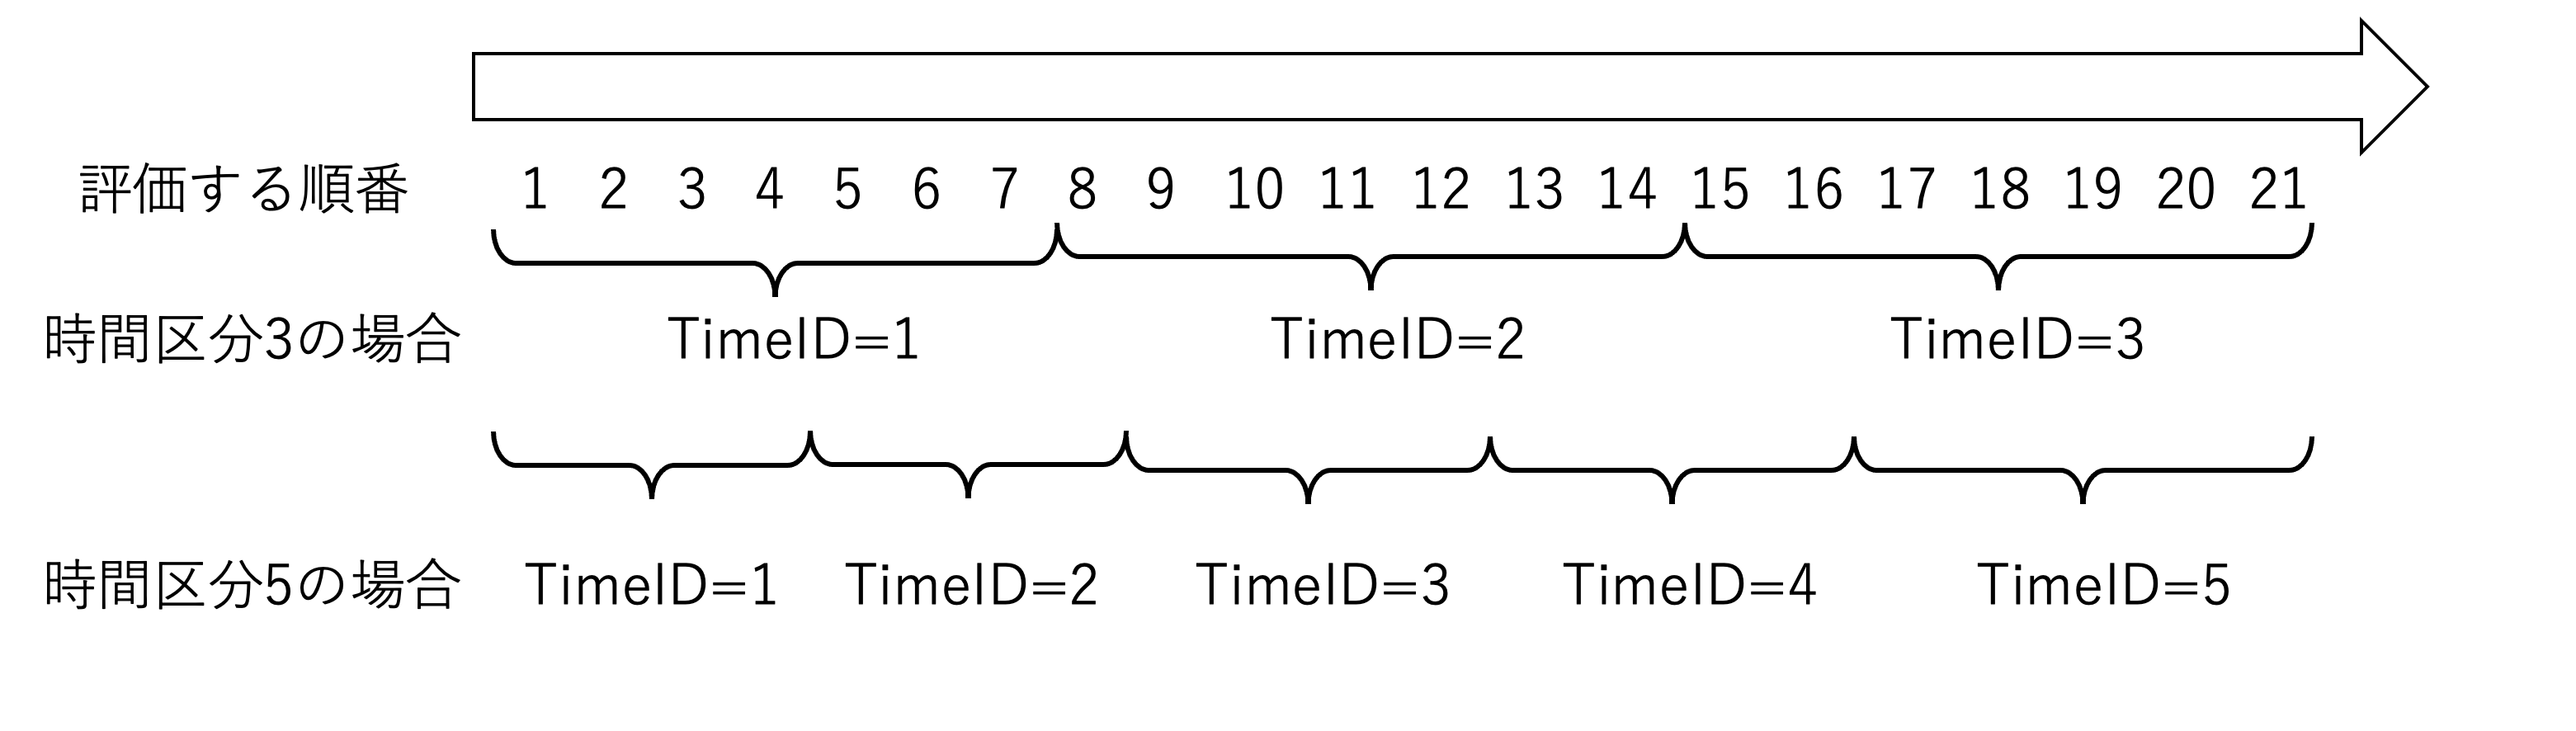
\includegraphics[width=8cm]{img/timeid.png}
  \caption{時間区分データのイメージと例}
  \label{timeid}
\end{figure}
このモデルは,パフォーマンス評価において,評価者と時間における評価者特性の変化を考慮することが可能である.しかし,このモデルの問題点として次の点が挙げられる.
(1)各時間区分ごとのパラメータが独立しているため,パラメータの推定が難しい.
(2)評価者の一貫性と各得点に対する基準の差異を考慮できていない.
以上の問題を解決するため,時間区分ごとの評価者の厳しさにマルコフ性を仮定した新しい項目反応モデルを次節で提案する.
\section{提案モデル}
提案モデルでは,受験者$j$のパフォーマンスに, 評価者$r$が時間区分$t$において評点$k$を与える確率$P_{jrtk}$を次式で定義する.
\begin{displaymath}
  P_{jrtk}=\frac{\mathrm{exp}\sum^k_{m=1}{\alpha_r(\theta_{j}-\beta_{rt}-d_{rm})}}{\sum^K_{l=1} \mathrm{exp}\sum^l_{m=1}{\alpha_r(\theta_{j}-\beta_{rt}-d_{rm})}}
\end{displaymath}
\begin{eqnarray}
  \beta_{rt}\sim \mathrm{N}(\beta_{r(t-1)},\sigma)\nonumber\\
  \beta_{r1} \sim \mathrm{N}(0,1)\nonumber\\
  \sigma \sim \mathrm{LN}(-3,0)\nonumber
\end{eqnarray}
ここで,$\alpha_{r}$は評価者$r$の一貫性,$\theta_{j}$は受験者$j$の能力,$\beta_{rt}は$評価者$r$の時間区分$t$における厳しさ,$d_{rk}$は評価者$r$からスコア$k$を得る困難度を示すステップパラメータである.

提案モデルでは,$\beta_{rt}$は,時間変化における評価者の厳しさの変化を表すため,$\beta_{r(t-1)}$に基づいて$\beta_{rt}$を決定されるように設計されている.そのため上記のように仮定する.
なお,$\sigma$の事前分布に$\mathrm{LN}(-3,0)$を設定した理由は次のとおりである.$\sigma$は0から1の間で,なおかつ,できる限り小さい値とすることで,$\beta_{rt}(t>1)$の事後分布が縮小するため,パラメータ推定が安定すると期待できる.上記を満たすような分布として,ここでは,$\mathrm{LN}(-3,0)$を採用した.

また,モデルの識別性のために,$\theta_{j}\sim N(0,1),\prod_{r}\alpha_r=1,d_{r1}=0,\sum_{k=2}^{K}d_{rk}=0$を仮定する.

本研究では提案モデルのパラメータ推定手法としてMCMC法を用いる.パラメータの事前分布は$\theta_{j},d_{rk},\mathrm{log}\alpha_{r},\beta_{rt}\sim N(0.0,1.0^{2})$とした.ここで,$N(\mu,\sigma^2)$は平均$\mu$,標準偏差$\sigma$の正規分布を表す.本研究では,MCMCのバーンイン期間は1000とし,1000$\sim$2000時点までの1000サンプルを用いる.
\section{シミュレーション実験}

本節では,MCMCアルゴリズムによる提案モデルのパラメータ推定精度をシミュレーション実験により評価する.実験手順は以下の通りである.
(1)パラメータの真値を,モデルの分布に従って生成する.
(2)手順(1)で生成したパラメータを用いて,データを生成する.
(3)手順(2)で生成したデータからパラメータ推定を行う.
(4)手順(3)で得られたパラメータ推定値と手順(1)で生成したパラメータ真値において,平均平方二乗誤差(RMSE)とバイアスを求める.
(5)以上を5回繰り返し実行し,RMSEとバイアスの平均値を求める.

上記の実験を,学習者数$j=50,100$,評価者数$r=10,15$,時間区間$t=3,5,10$の場合において行った.カテゴリ数は$K=5$とした.
実験結果を表\ref{parameters_recovery}に示す.

\begin{table}[t]
  \begin{minipage}[t]{8cm}
    \centering
    \caption{パラメータ・リカバリ実験の結果}
    \setlength{\tabcolsep}{5.pt}
    \scalebox{0.8}{
      \begin{tabular}{cccccccccccccc}  
        \bhline{1pt}
        \multirow{2}{*}{$J$} & \multirow{2}{*}{$R$} & \multirow{2}{*}{$T$}  && \multicolumn{4}{c}{RMSE} &&   \multicolumn{4}{c}{BIAS}  \\
        \cline{5-8}\cline{10-13}
          & & & & $\theta$ & $\alpha_r$ & $\beta_{rt}$ & $d_{rk}$ &  & $\theta$ & $\alpha_r$ & $\beta_{rt}$ & $d_{rk}$ \\
        \bhline{1pt}
        50 & 10 & 3 & & 0.24 & 0.27 & 0.20 & 0.40 & &0.02  & 0.02 & 0.06  & 0.00 \\
          &   & 5  && 0.30 & 0.24 & 0.31 & 0.38 & &-0.01 & -0.00 & -0.03 & -0.00  \\
          &   & 10 && 0.32 & 0.36 & 0.36 & 0.41 && 0.01  & 0.04 & -0.02 & 0.00 \\
        \cline{2-14}
        & 15 & 3  && 0.25 & 0.30 & 0.25 & 0.37 && 0.03 & 0.01 & 0.06 & 0.00  \\
        &  & 5  && 0.25 & 0.23 & 0.19 & 0.34 && 0.03 & 0.01 & 0.01 & -0.00  \\
        &  & 10 && 0.24 & 0.26 & 0.33 & 0.39 && 0.02 & 0.02 & 0.03 & 0.00 \\
        \hline
        100 & 10 & 3  && 0.26 & 0.19 & 0.13 & 0.28 && -0.02 & 0.00 & -0.01 & 0.00  \\
        &  & 5  && 0.27 & 0.19 & 0.13 & 0.27 && 0.01  & 0.00 & 0.00  & 0.00  \\
        &  & 10 && 0.26 & 0.18 & 0.19 & 0.30 && -0.02 & 0.02 & -0.03 & -0.00 \\
        \cline{2-14}
        & 15 & 3  && 0.23 & 0.22 & 0.20 & 0.30 && 0.00 & 0.02 & 0.00 &0.00 \\
        &  & 5  && 0.23 & 0.20 & 0.18 & 0.31 && 0.03 & 0.01 & 0.06  &0.00\\
        &  & 10 && 0.24 & 0.25 & 0.40 & 0.38 && 0.01 & 0.02 & -0.01 &0.00\\
        \hline
        \multicolumn{4}{c}{Avg.}   &  0.26 & 0.24 & 0.24 & 0.34 &  & 0.01 & 0.01 & 0.01 & 0.00 & \\
        \bhline{1pt}
      \end{tabular}
    }
    \label{parameters_recovery}
  \end{minipage}
\end{table}

表\ref{parameters_recovery}から,関連研究と同様に,学習者数・評価者数の増加に伴い推定精度が改善する傾向が読み取れる.また時間区分の総数Tが多くなると性能が低下する傾向も読み取れる.これはパラメータ数に対するデータ数が減少するためと考えられる.

また,$\beta_{rt}$のパターンごとの推定結果の例を図\ref{beta_rt_data}に示す.縦軸が$\beta_{rt}$,横軸がTimeIDであり,実線が作成したパラメータ真値,点線が推定したパラメータである.このグラフより,作成した真値にある程度従って,パラメータが推定されていることがわかる.

以上の結果から, MCMCにより提案モデルのパラメータを適切に推定できることが確認できた.

\section{実データ実験}
本章では,実データの適用を通して,提案モデルの有効性を評価する.

本研究では,34名の被験者にエッセイ課題を与え,そのエッセイを34名の評価者が5段階得点で採点したデータを使用する.
本研究では,このデータに対して提案モデルを適用する.

実データから推定された$\beta_{rt}$の例を,図\ref{beta_rt_data}に示す.縦軸が$\beta_{rt}$,横軸がTimeIDである.赤色の実線で示した評価者は評価中に厳しさが減少しており,緑色の実線で示した評価者は評価中に厳しさが増加している.対して青色の実線で示した評価者は評価中にあまり厳しさが変化していないことがわかる.

\begin{figure}[t]
  \begin{minipage}[b]{4cm}
    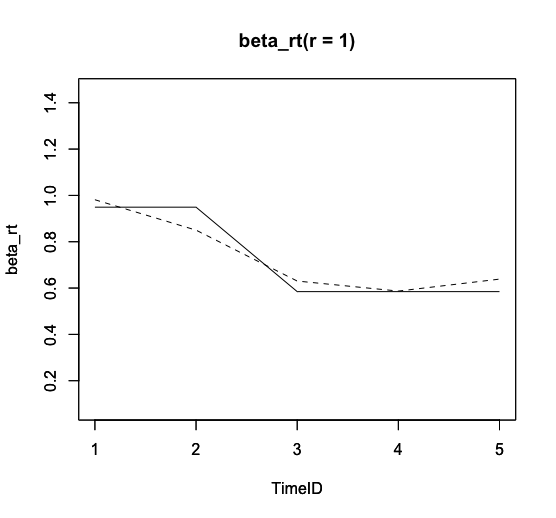
\includegraphics[keepaspectratio, scale=0.22]{img/beta_rt_param.png}
   % \subcaption{シミュレーション実験の結果例}
  \end{minipage}
  \begin{minipage}[b]{4cm}
    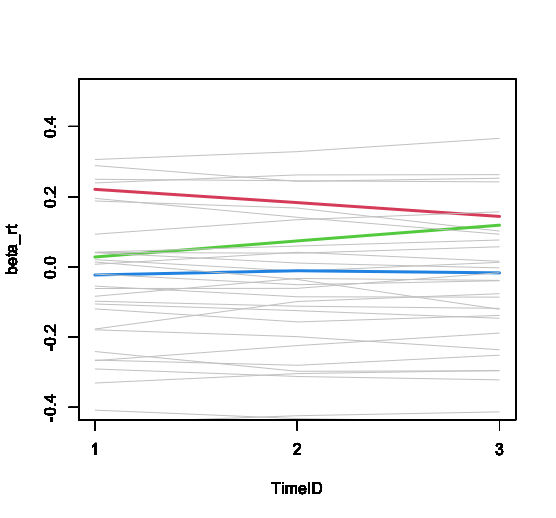
\includegraphics[keepaspectratio, scale=0.22]{img/beta_rt_data.png}
   % \subcaption{実データ実験の結果}
  \end{minipage}
 %  \vspace*{0.5cm}
  \caption{$\beta_{rt}$の推定結果の例}
  \label{beta_rt_data}
  \vspace*{0.5cm}
\end{figure}

以降では,提案モデルの性能を評価するために,\textbf{2.}で紹介した既存モデルとの性能比較を行う.

本節では,情報量規準によるモデル比較により提案モデルの性能を評価する.ここでは, MCMCにより各モデルのパラメータを推定し,得られた推定値を用いて情報量規準を求めた.情報量規準にはMCMCのパラメータサンプルから算出できるWAIC(Widely Applicable Information Criterion)とWBIC(Widely Applicable Bayesian Information Criterion)を用いた.ここで,WAICは将来のデータの予測に優れたモデルを選択する規準である.他方で,WBICは真のモデルを漸近的に選択できる基準である.どちらの場合も,値が小さい方が適したモデルであるということを示す.

実験結果を表\ref{WAICWBIC}に示す.縦軸は使用したデータの時間区分であり,横軸は各モデルのWAIC,WBICの値である.

\begin{table}[t]
  \centering
  \begin{minipage}[t]{9cm}
    \centering
    \caption{モデル比較の結果}
    \setlength{\tabcolsep}{5.pt}
    \begin{tabular}{cccccccc}  
      \bhline{1pt}
      &時間区分  &既存モデル & 提案モデル \\ 
      \bhline{1pt}
      WAIC &3    & 3106.633 & \textbf{2956.466} \\
      &5    & 3171.920 & \textbf{2962.159} \\
      &10   & 3296.762 & \textbf{2961.461} \\
      \bhline{1pt}
      WBIC&3    & 1825.648 & \textbf{1808.674} \\
      &5    & 1916.035 & \textbf{1807.423} \\
      &10   & 2016.664 & \textbf{1806.655} \\
      \bhline{1pt}
    \end{tabular}
    \label{WAICWBIC}
  \end{minipage}
\end{table}

表\ref{WAICWBIC}から,各時間区分におけるWAICとWBICの最小値を比較すると,提案モデルが最適モデルとして選択されたことが確認できる.

\section{まとめと今後の課題}
本研究では,時間区分ごとの評価者の厳しさにマルコフ性を仮定した新しい項目反応モデルを提案した.また,シミュレーション実験と実データを用いた実験を通して,提案モデルの有効性を示した.
今後の課題として,以下のものがある.
\begin{itemize}
  \item さらに多くの評価者データを集めて推定を行う.
  \item 課題特性も考慮して推定を行う.
  \item 既存モデルとの比較をさらに細かく行う.
\end{itemize}

{\small
\bibliographystyle{chukan}
\bibliography{chukan}
}
\end{document}